\subsection{Payment Channel Management}
\label{sec:incentives:channels}

For node $A$ to transfer packets to node $B$, it must first open a payment channel. There are four distinct payment channel states, represented in the following scheme:

\begin{figure}[H]
    \centering
    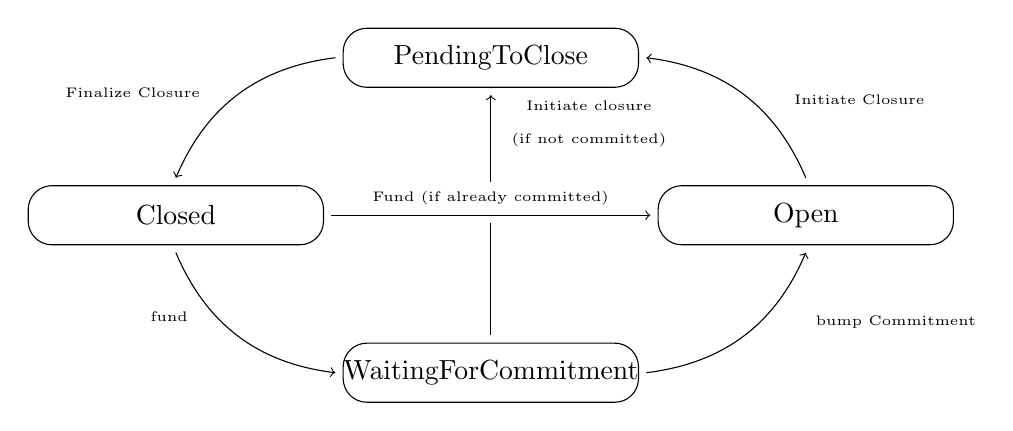
\begin{tikzpicture}[every text node part/.style={align=center}]
        \def\nodeWidth{3.75}
        \def\nodeHeight{0.75}
        \def\padding{0.1}
        \foreach \posX\posY\tag in{0/0/Closed,4/2/PendingToClose,8/0/Open,4/-2/WaitingForCommitment} {
                \draw[rounded corners=3mm,shift={(\posX,\posY)}] (0,0) rectangle (\nodeWidth,\nodeHeight) node[midway] {\smaller{\tag}};
            }

        \draw[->] (4-\padding,2+\nodeHeight/2) to [bend right] (\nodeWidth/2,\nodeHeight+\padding) node[midway,above=55pt,right=10pt] {\tiny{Finalize Closure}};
        \draw[->] (8+\nodeWidth/2,\nodeHeight+\padding) to [bend right] (4+\nodeWidth+\padding,2+\nodeHeight/2) node[below=15pt,right=50pt] {\tiny{Initiate Closure}};
        \draw[->] (\nodeWidth/2,0-\padding) to [bend right] (4-\padding,-2+\nodeHeight/2) node[left=60pt,above=15pt] {\tiny{fund}};
        \draw[->] (4+\nodeWidth+\padding,-2+\nodeHeight/2) to [bend right] (8+\nodeWidth/2,0-\padding) node[below=25pt,right=0.1pt] {\tiny{bump Commitment}};

        \draw (4+\nodeWidth/2,-2+\nodeHeight+\padding) -- (4+\nodeWidth/2,\nodeHeight/2-\padding);
        \draw[->] (4+\nodeWidth/2,\nodeHeight/2+\padding) -- (4+\nodeWidth/2,2-\padding) node[midway,above=10pt,right=4pt] {\tiny{Initiate closure}\\\tiny{(if not committed)}};
        \draw[->] (\nodeWidth+\padding,\nodeHeight/2) -- (8-\padding,\nodeHeight/2) node[midway,fill=white,above=0.2pt] {\tiny{Fund (if already committed)}};
    \end{tikzpicture}
    \caption{Payment channel states}
\end{figure}

Initially, each payment channel is \textit{Closed}.

\paragraph{Opening a channel} Node $A$ can open a channel by transferring funds to the payment channels contract \textit{HoprChannels} and including the following \textit{userdata}:

$$[A: address, B: address, \lambda: uint8, \mu: uint8], \mu = 0,$$

where $\lambda$ is the amount to be staked by $A$. This call will trigger an on-chain event \textit{ChannelFunded} and open a unidirectional payment channel from $A$ to $B$. The payment channel will start in state \textit{Waiting for commitment}. The destination address of the payment channel must now set an on-chain commitment in order for the payment channel between both parties to become \textit{Open}. This is done by $B$ calling the \textit{bumpChannel()} function to make a new set of commitments towards this payment channel. This call will trigger an on-chain event \textit{ChannelOpened} and bumps the ticket epoch to ensure tickets with the previous epochs are invalidated. Every time the channel changes its state, an on-chain event \textit{ChannelUpdated} is emitted.

\paragraph{Redeeming tickets}
As long as the channel remains open, nodes can claim their incentives for forwarding packets via tickets. Tickets are redeemed by dispatching a \textit{redeemTicket()} call to an \textit{Open} payment channel.

If $B$ tries to redeem a ticket from the channel $A\rightarrow B$ (spending channel), but there is an open channel $B\rightarrow A$ (earning channel), $B$'s rewards will be transferred to $B\rightarrow A$ (earning channel). Otherwise, rewards will be sent directly to $B$.

\paragraph{Closing a channel}
Nodes can close a payment channel in order to access their previously staked funds. Only the payment channel creator can initiate the process by calling \textit{initiateChannelClosure()}. This changes the state to $Pending to close$ and triggers a grace period during which the destination node can redeem any unredeemed tickets. Nodes should actively monitor blockchain events to be aware of this payment channel state change.

Once the grace period has elapsed, the payment channel creator can call \textit{finalizeChannelClosure()} which changes the payment channel to $Closed$. When a payment channel is closed, the remaining funds are automatically transferred to the payment channel creator. The channel epoch increments, meaning any unredeemed tickets can no longer be redeemed.
